%------------------------------------------------
\begin{frame}
\frametitle{Wellbeing is a process of choice}
\hypertarget{posture}{}
\begin{columns}[c] % The "c" option specifies centered vertical alignment while the "t" option is used for top vertical alignment

\column{.3\textwidth} % Left column and width

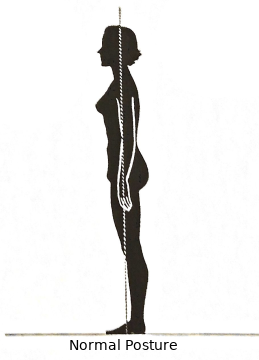
\includegraphics[width=\linewidth]{Normal_Posture}

\column{.7\textwidth} % Left column and width
We try out movements and wonder: does that \structure{work better}? Is this movement more fluent? This process can lead too problems while being in a state of fear, pain or stress.
We then choose the movements we know and bring us relief.

Paradoxically we subconsciously choose \structure{stiff and tensed up movements}. We don't swing the hips any more, choose confining movements, contract belly and chest and hold the head and neck in a rigid position.
Choosing such habits, we \structure{invite difficulties} into our lives.

\structure{Well--being} is therefore a question of knowledge, attitude, our actions and our joy of life. Our movements influence our whole life.
\end{columns}

\end{frame}
%------------------------------------------------
%------------------------------------------------
\begin{frame}
\frametitle{Malposition as permanent stress}
\begin{columns}[c] % The "c" option specifies centered vertical alignment while the "t" option is used for top vertical alignment

\column{.4\textwidth} % Left column and width

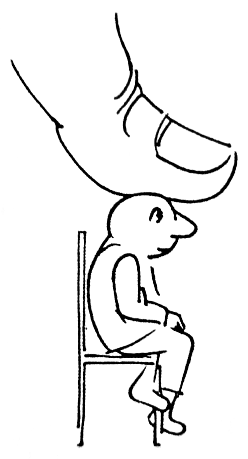
\includegraphics[width=\linewidth]{Thumb_head}

\column{.6\textwidth} % Left column and width
The malposition, a wrong posture, is regarded as the \structure{most basic afferent} (from the outside to the brain) impulse for many afflictions of many people. 

Given that the posture influences the psyche of a human being, the physiological posture is important to \structure{center the mind}. 
\end{columns}

\end{frame}
%------------------------------------------------
%------------------------------------------------
\begin{frame}
\frametitle{A good, straight posture}
\begin{columns}[c] % The "c" option specifies centered vertical alignment while the "t" option is used for top vertical alignment

\column{.3\textwidth} % Left column and width

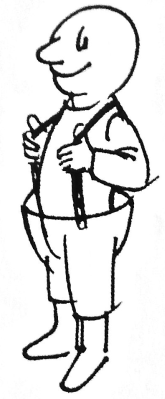
\includegraphics[width=0.8\linewidth]{Smiling_Guy}

\column{.6\textwidth} % Left column and width
A good posture only needs a \structure{minimal muscle effort to move} the body easily. That means that with a good posture no real muscle effort is necessary, because the parts of the skeleton are \structure{balanced} and as close as possible from the \structure{central axis}. 

In the ideal posture, there's exactly the \structure{same tension} on the outer (movement related) muscles and the inner musculature.
\note{Beside the shape of the spine, the mental sate, the state of the musculature and the physical constitution should be considered for an evaluation of the posture.}
\end{columns}

\end{frame}
%------------------------------------------------
%------------------------------------------------
\begin{frame}
\frametitle{The physiological posture}
\begin{columns}[c] % The "c" option specifies centered vertical alignment while the "t" option is used for top vertical alignment

\column{.3\textwidth} % Left column and width

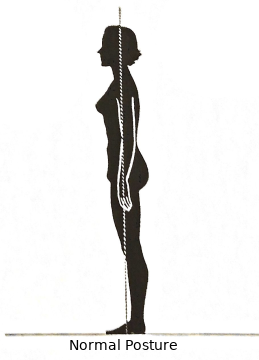
\includegraphics[width=1.2\linewidth]{Normal_Posture}

\column{.6\textwidth} % Left column and width
Which posture is needed to avoid the strain on the structures of the body, which act as disturbances? The main tell tale sign of a good posture is an \structure{even lordosis} (concave curvature of the spine between central thoracic spine and the sacrum).

The lumbar lordosis (hollow--back) is harmful, if it isn't \structure{pulled up to the middle of the thoracic spine}. In this position, the spine can carry the body. The lumbar bone connects in a harmonious arc with the fifth thoracic vertebra between the shoulder blades to carry out its structural function.
\end{columns}

\end{frame}
%------------------------------------------------
